\documentclass[aspectratio=169,10pt]{beamer}
\usepackage{../assets/acemoglu-beamer}
\title[AKO (2026): auditoría]{AI, Human Cognition and Knowledge Collapse}
\subtitle{Cómo funciona el mecanismo, qué mide el bienestar y dónde falla la robustez}\author{Belén Vásquez}\date{Septiembre de 2026}
\begin{document}
\begin{frame}[plain]\titlepage\begin{center}\paperref\\\href{\RepoURL}{\texttt{github.com/sbvasquezg-ux/ai-04-acemoglu}}\end{center}\end{frame}
\begin{frame}{Pregunta y ruta del argumento}
\textbf{Pregunta central.} ¿Puede una IA que mejora las decisiones privadas terminar destruyendo el conocimiento público que hace valiosas esas decisiones?
\begin{enumerate}\item Definir qué representan $X$, $Y$, $e$ y $\tau_A$.\item Mostrar por qué $X$ complementa el esfuerzo y $\tau_A$ lo sustituye.\item Seguir el efecto de menor esfuerzo sobre $X_{t+1}$.\item Separar el beneficio inmediato de la pérdida dinámica de bienestar.\item Probar qué parte del colapso depende de supuestos de frontera.\end{enumerate}
\keybox{Objetivo de la presentación: reconstruir el resultado y defender una objeción de robustez, no resumir todo el paper.}
\sourcefoot{Introducción y \S\S3--5, pp. 2--33.}\end{frame}
\begin{frame}{La producción impone complementariedad extrema}
\[
\Delta_G=f(1,0)-f(0,0),\quad\Delta_I=f(0,1)-f(0,0),\quad
\Delta_X=f(1,1)-f(1,0)-f(0,1)+f(0,0).
\]
\textbf{Assumption 1:} $\Delta_I=0$, $\Delta_X>0$; además $\Delta_G+\Delta_I+\Delta_X=1$. El ejemplo Leontief fija $\Delta_G=\Delta_I=0$, $\Delta_X=1$.
\keybox{Contexto específico sin conocimiento general no añade output: esta frontera vuelve posible bienestar cero.}
\sourcefoot{§3.1, pp. 8--10.}\end{frame}
\begin{frame}{Información y dominios}
\begin{align*}\theta_{t+1}&=\theta_t+\epsilon_t,&&\epsilon_t\sim N(0,\Sigma^2),\\
\theta_{i,t}&\sim N(0,\sigma^2),&s^H_{i,t}&\sim N(\theta_{i,t},(\lambda_Ie)^{-1}),\\
s^A_{i,t}&\sim N(\theta_{i,t},\tau_A^{-1}),&s^C_t&\sim N(\theta_t,(\lambda_GE_t)^{-1}).\end{align*}
$e\ge0$, $\tau_A\ge0$, $\lambda_I,\lambda_G>0$, $\alpha>1$, $I\in[1,M]$.
\sourcefoot{§3.1, pp. 8--12.}\end{frame}
\begin{frame}{Problema estático y CPO}
\[
U=f(0,0)+G(X)\Delta_G+G(X)G(\sigma^{-2}+\lambda_Ie+\tau_A)\Delta_X-e^\alpha/\alpha.
\]
\[
U_e=\Delta_XG(X)\lambda_Ig(Y)-e^{\alpha-1}=0.
\]
\begin{itemize}\item $e$: esfuerzo cognitivo elegido por la persona; $X$: precisión del conocimiento general heredado.
\item $Y=\sigma^{-2}+\lambda_Ie+\tau_A$: precisión contextual total; $\tau_A$ es la parte que entrega la IA.
\item $G(z)$ es la probabilidad de una decisión correcta; $e^\alpha/\alpha$ es el costo de pensar.
\end{itemize}
$g$ decrece y el costo marginal crece: máximo único. Para $X>0$ es interior; para $X=0$, $e^*=0$.
\sourcefoot{Ecuaciones (4)--(6), §3.5 y nota 4, pp. 12--15.}\end{frame}
\begin{frame}{Observación 1: prueba y frontera}
\[
U_{eX}=\Delta_X\lambda_Ig(X)g(Y)>0,\qquad
U_{e\tau_A}=\Delta_XG(X)\lambda_Ig'(Y)<0.
\]
\begin{itemize}\item $U_{eX}>0$: $X$ y $e$ son complementos; más base común vuelve más productivo el esfuerzo individual.\item $U_{e\tau_A}<0$: $\tau_A$ y $e$ son sustitutos; la IA aporta la precisión que la persona obtendría pensando.\item Menos $e$ también reduce la señal que la sociedad agrega en $X_{t+1}$, efecto que el individuo no internaliza.\item En $X=0$, la segunda desigualdad es cero y la primera derivada no es finita.\end{itemize}
\sourcefoot{Observación 1, §3.4, pp. 13--14; nota 4, p. 15.}\end{frame}
\begin{frame}{Del esfuerzo al estado estacionario}
\[
X_{t+1}=F(X_t)=\left[\Sigma^2+(X_t+\lambda_GIe(X_t,\tau_A))^{-1}\right]^{-1}.
\]
\begin{itemize}\item $E_t=I e_t$ es esfuerzo total; $\lambda_GE_t$ mide cuánta precisión pública produce la cohorte.\item $F(X_t)$ transforma el conocimiento actual y la nueva señal en el stock del próximo período.\item Si $1/(\alpha-1)>4$, el esfuerzo responde mucho a incentivos y cero es localmente estable; si es menor que cuatro, cero es inestable.\item La igualdad no queda clasificada por Lemma 2.
\end{itemize}
\sourcefoot{Ecuaciones (7)--(9), Lemma 2, pp. 16--18.}\end{frame}
\begin{frame}{Colapso completo requiere más que Observación 1}
Para elasticidad mayor que cuatro, puede haber tres steady states. Si $\tau_A>\tau_A^c$, queda solo $\bar X=0$ y es globalmente estable.
\begin{itemize}\item Atomisticidad: nadie internaliza la señal pública.\item $\Delta_I=0$: la señal privada sola vale cero.\item Sin flujo autónomo: $F(0)=0$.\end{itemize}
\sourcefoot{Proposición 5, §§3.7--3.8, pp. 19--23.}\end{frame}
\begin{frame}{Bienestar: una derivada con dos signos}
\[
\bar U=G(\bar X)\Delta_G+G(\bar X)G(\bar Y)\Delta_X-\bar e^\alpha/\alpha,
\]
\[
\bar U_{\tau_A}=
\underbrace{g(\bar Y)G(\bar X)\Delta_X}_{DE\ge0}+
\underbrace{G_{\tau_A}(\bar X)[\Delta_G+G(\bar Y)\Delta_X]}_{-IE\le0}.
\]
\begin{itemize}\item $DE$: mejor consejo aumenta hoy la probabilidad de elegir correctamente.\item $IE$: una mayor $\tau_A$ reduce esfuerzo, agregación y el stock estacionario $\bar X$; por eso $G_{\tau_A}(\bar X)<0$.\item El signo total depende de cuál de los dos canales domina.
\end{itemize}
\sourcefoot{Ecuación (10), §4.3, pp. 24--26.}\end{frame}
\begin{frame}{Lectura de la curva de bienestar}\small
\begin{columns}[T,onlytextwidth]\column{.58\textwidth}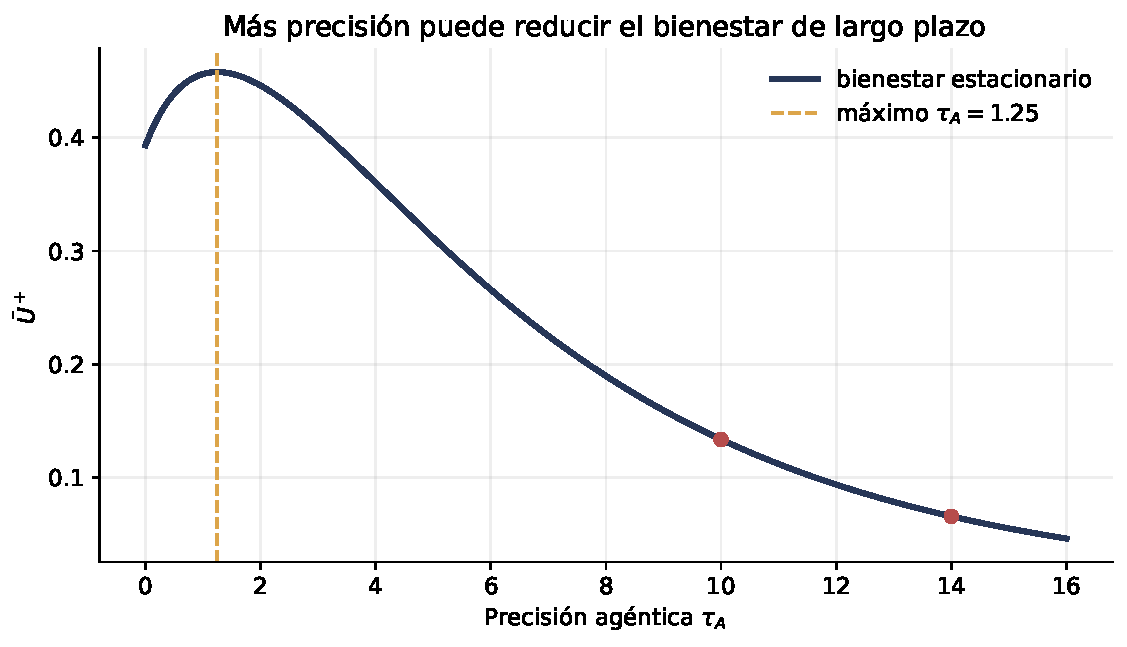
\includegraphics[width=\linewidth]{figures/welfare-accuracy.pdf}\column{.39\textwidth}\begin{itemize}\item \textbf{Eje horizontal:} $\tau_A$, precisión de la recomendación agéntica.\item \textbf{Eje vertical:} $\bar U^+$, utilidad neta en el estado estacionario alto.\item Antes de $\tau_A^\star$ domina el beneficio directo.\item Después domina la pérdida de conocimiento general y la utilidad cae estrictamente.\item Assumption 2 evita cambios múltiples de signo.\end{itemize}\end{columns}
\keybox{La figura no dice que ``la IA empeora el bienestar'' en general. Dice que, dentro del modelo y a partir de un umbral, una mejora marginal de precisión destruye más valor dinámico del que crea hoy.}
\sourcefoot{Proposiciones 10--11, pp. 26--27; simulación propia.}\end{frame}
\begin{frame}{Las seis relajaciones: qué sí está en el PDF}
\scriptsize
\begin{tabular}{p{.29\linewidth}p{.63\linewidth}}\toprule Candidato&Resultado de auditoría\\\midrule
IA agrega general&Relajado en §5.1; sobrevive solo si $\eta<1/[2(\alpha-1)]$.\\
Datos sintéticos&Relajado en §5.2; $\tau_{syn}>0$ elimina el steady state cero.\\
$\tau_A(X)$&No modelado; signo total ambiguo.\\
CES&No modelado; la tabla binaria con $\Delta_I=0$ no es CES.\\
Entrada/especialistas&No hay precio ni heterogeneidad de costo; simetría impuesta.\\
Aprendizaje usando IA&No hay stock individual persistente; cohortes cortas e idiosincrasia i.i.d.\\\bottomrule\end{tabular}
\sourcefoot{§§3.1, 5.1--5.3, pp. 8--12 y 30--33.}\end{frame}
\begin{frame}{Comparación con Quispe--Xu (2026)}
\begin{itemize}\item El portafolio de lenguajes crece persistentemente tras adopción.\item El patrón sobrevive al excluir commits coescritos por el agente.\item Es compatible con aprendizaje y complementariedad, no prueba causal definitiva por adopción voluntaria.\end{itemize}
\keybox{Añadir aprendizaje persistente rompe la equivalencia entre ``menos esfuerzo hoy'' y ``menos capacidad humana mañana''.}
\sourcefoot{Quispe \& Xu (2026), abstract/resultados reportados; contraste propio con §3.1 de AKO.}\end{frame}
\begin{frame}{Veredicto y comprobación manuscrita}
\begin{columns}[T,onlytextwidth]\column{.60\textwidth}
\begin{block}{Sobrevive}Más precisión contextual puede reducir esfuerzo, conocimiento general y bienestar; con elasticidad alta puede haber trampas y path dependence.\end{block}
\begin{block}{No sobrevive sin condiciones}``Todo conocimiento desaparece'': con $\Delta_I>0$ o $\tau_{syn}>0$, cero deja de ser punto fijo.\end{block}
\keybox{Enunciado defendible: la IA puede desplazar la economía hacia conocimiento bajo; cero exacto es una propiedad del baseline.}
\column{.36\textwidth}\centering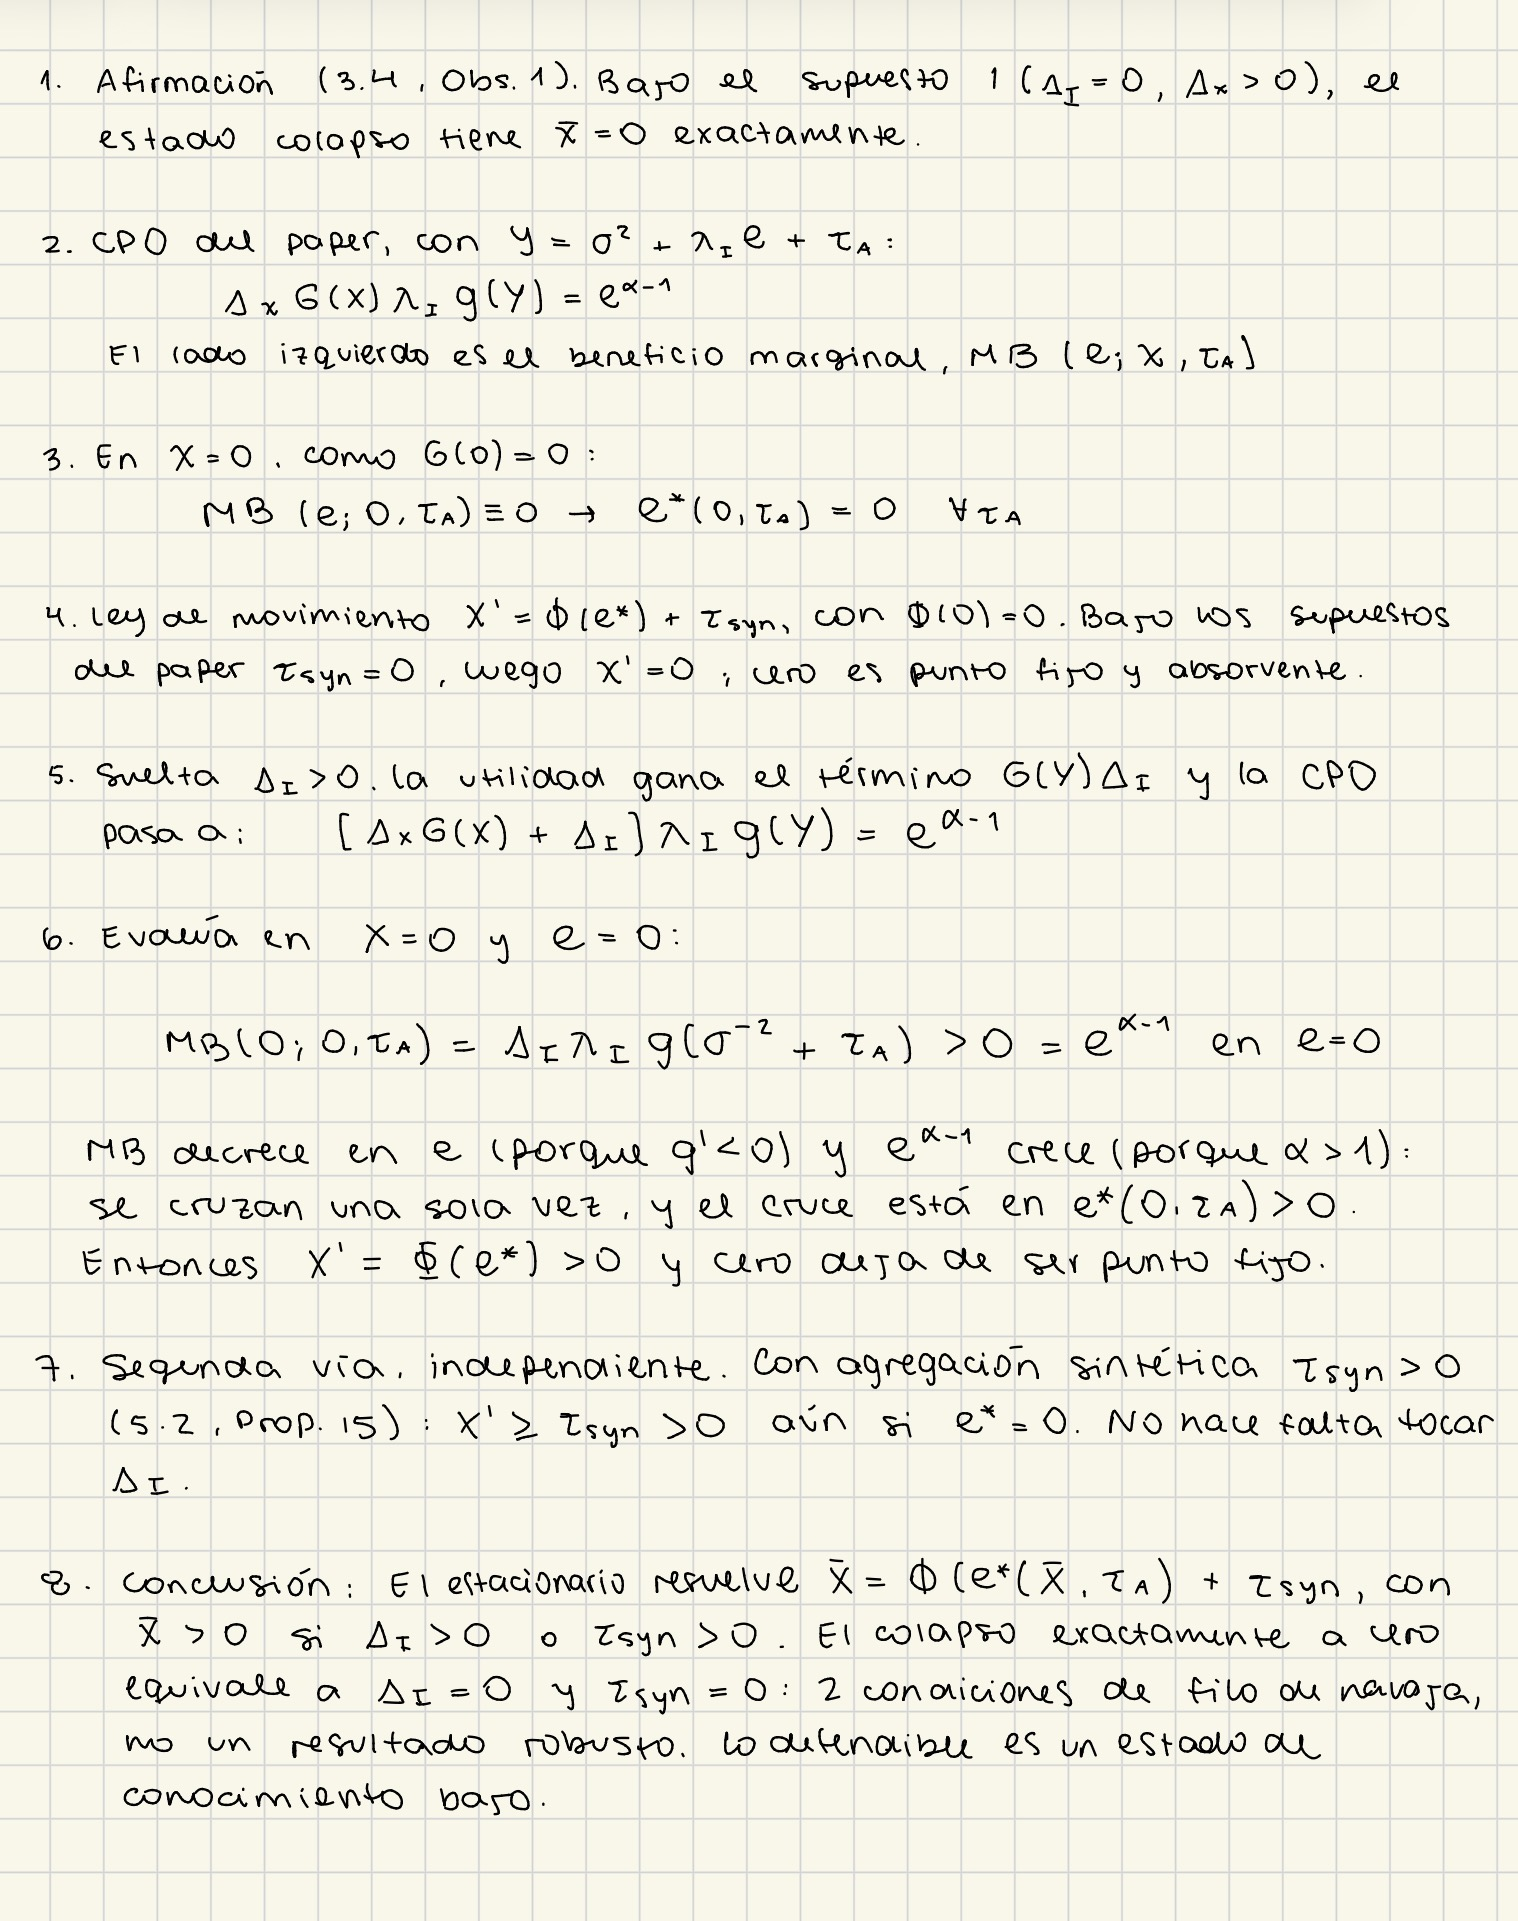
\includegraphics[width=\linewidth,height=.62\textheight,keepaspectratio]{../hand/manual-verification.jpg}\\\scriptsize Evidencia aportada por la estudiante.
\end{columns}
\sourcefoot{Assumption 1 y Proposiciones 5, 10--11 y 15, pp. 9, 21--27 y 32.}\end{frame}
\end{document}
